\message{ !name(calculus.tex)}
\message{ !name(calculus.tex) !offset(-2) }
%Master File:lectures.tex


\lesson{Calculus}
\vspace{-1cm}
\begin{center}
  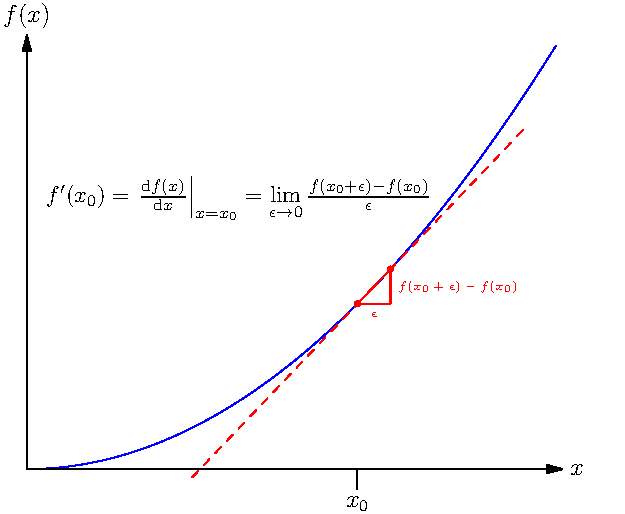
\includegraphics[height=10cm]{derivative-2}
\end{center}
\keywords{Differentiation, Integration}
%%%%%%%%%%%%%%%%%%%%%%% Next Slide %%%%%%%%%%%%%%%%%%%%%%%
\renewcommand{\Outline}{%
\begin{slide}
\section[1]{Outline}

\begin{minipage}{10cm}\raggedright
  \begin{enumerate}\squeeze
    \outlineitem{Why Calculus?}{calculus}
    \outlineitem{Differentiation}{differentiation}
    \outlineitem{Integration}{integration}
  \end{enumerate}
\end{minipage}\hfill
\begin{minipage}{12cm}
  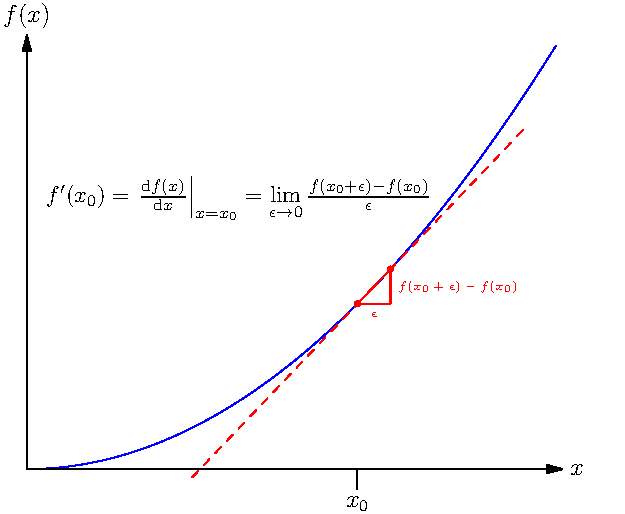
\includegraphics[width=12cm]{derivative-2}
\end{minipage}
\end{slide}
\addtocounter{outlineitem}{1}
}

\newcommand{\bits}{\,\mathrm{bits}}
\setcounter{outlineitem}{1}


%%%%%%%%%%%%%%%%%%%%%%% Next Slide %%%%%%%%%%%%%%%%%%%%%%%
\Outline % Why Calculus
%%%%%%%%%%%%%%%%%%%%%%% Next Slide %%%%%%%%%%%%%%%%%%%%%%%

\begin{slide}
\section{Why Calculus?}

\begin{PauseHighLight}
  \begin{itemize}
  \item Calculus is a fundamental tool of mathematical analysis\pause
  \item In machine learning differentiation is fundamental tool in
    optimisation\pause
  \item Integration is an essential tool in taking expectations over
    continuous distributions\pause
  \item Both differentiation and integration crop up elsewhere\pause
  \item This material will not be examined explicitly\pauseb, but I
    assume elsewhere that you can do calculus\pauseb
  \end{itemize}
\end{PauseHighLight}

\end{slide}

%%%%%%%%%%%%%%%%%%%%%%% Next Slide %%%%%%%%%%%%%%%%%%%%%%%

\begin{slide}
\section{Back to Basics}
  
\begin{PauseHighLight}
  \begin{itemize}
  \item You have all done A-level maths so should be familiar with the
    rules of calculus\pause
  \item But, it is easy to forget the rules and sometimes we use quite
    sophisticated tricks\pause
  \item Although the sophisticated tricks really speed up
    calculations, it pays to be able to understand where these tricks
    come from\pause
  \end{itemize}
\end{PauseHighLight}

\end{slide}

%%%%%%%%%%%%%%%%%%%%%%% Next Slide %%%%%%%%%%%%%%%%%%%%%%%
\Outline % Differentiation
%%%%%%%%%%%%%%%%%%%%%%% Next Slide %%%%%%%%%%%%%%%%%%%%%%%

\begin{slide}
  \section[-1]{Differentiation}

  \pb \pause \pauselevel{=1}
  \begin{center}
    \multipdf[width=0.7\linewidth]{derivative}\pause
  \end{center}

\end{slide}

%%%%%%%%%%%%%%%%%%%%%%% Next Slide %%%%%%%%%%%%%%%%%%%%%%%

\begin{slide}
\section{Polynomials}

\begin{PauseHighLight}
  \begin{itemize}
  \item $f(x)=x^2$
    \begin{align*}
      \frac{\dd x^2}{\dd x} &= \lim_{\epsilon\rightarrow 0}
      \frac{(x+\epsilon)^2 - x^2}{\epsilon}\pause
      =  \lim_{\epsilon\rightarrow 0}
      \frac{(x^2 + 2\,\epsilon\,x + \epsilon^2) -
                              x^2}{\epsilon}\pauseb
                              \\
      &= \lim_{\epsilon\rightarrow 0} 2\,x + \epsilon\pauseb = 2\,x\pauseb
    \end{align*}
  \item $(x+\epsilon)^n =
    (x+\epsilon)(x+\epsilon)\cdots(x+\epsilon)\pauseb = x^n +
    n\,\epsilon\,x^{n-1} + O(\epsilon^2)$\pauseb
     \begin{align*}
      \frac{\dd x^n}{\dd x} &= \lim_{\epsilon\rightarrow 0}
      \frac{(x+\epsilon)^n - x^n}{\epsilon}\pauseb
      =   \lim_{\epsilon\rightarrow 0} n\,x^{n-1} + O(\epsilon)\pauseb = n\,x^{n-1}\pauseb
    \end{align*}
  \end{itemize}
\end{PauseHighLight}

\end{slide}

%%%%%%%%%%%%%%%%%%%%%%% Next Slide %%%%%%%%%%%%%%%%%%%%%%%

\begin{slide}
\section{Linearity of derivatives}
  
\begin{PauseHighLight}
  \begin{itemize}
  \item Note that $f(x+\epsilon) = f(x) + \epsilon\, f'(x) +
    O(\epsilon^2)$ (from the definition of $f'(x)$)\pause
    \begin{align*}
      \frac{\dd \bra{a\,f(x)+b\,g(x)}}{\dd x}
      &=
      \lim_{\epsilon\rightarrow 0}
      \frac{\bra{a\,f(x+\epsilon)+b\,g(x+\epsilon)}-\bra{a\,f(x)+b\,g(x)}}{\epsilon}
      \pause \\
      &=  \lim_{\epsilon\rightarrow 0}
        \frac{a\,\epsilon\, f'(x) +b\,\epsilon\,g'(x) +
        O(\epsilon^2)}{\epsilon}\pauseb \\
      &= a\,f'(x) + b\,g'(x) \pauseb
    \end{align*}
  \item \emph{Differentiation is a linear operation!}\pauseb
  \end{itemize}
\end{PauseHighLight}

\end{slide}

%%%%%%%%%%%%%%%%%%%%%%% Next Slide %%%%%%%%%%%%%%%%%%%%%%%

\begin{slide}
\section[-1]{Linearity in Pictures}

 \pb \pause \pauselevel{=1}
  \begin{center}
    \multipdf[width=0.8\linewidth]{difflinearity}\pause
  \end{center}

\end{slide}

%%%%%%%%%%%%%%%%%%%%%%% Next Slide %%%%%%%%%%%%%%%%%%%%%%%

\begin{slide}
  \section{Product Rule}

\begin{PauseHighLight}
  \begin{itemize}
  \item Recall $f(x+\epsilon) = f(x) + \epsilon\, f'(x) + O(\epsilon^2)$
  \item If $h(x) = f(x)\, g(x)$\pause
    {\small
    \begin{align*}
      h'(x) &= \lim_{\epsilon\rightarrow 0}
      \frac{f(x+\epsilon)\,g(x+\epsilon)-f(x)\,g(x)}{\epsilon}\pauseb \\
      &= \lim_{\epsilon\rightarrow 0} \frac{\bra{f(x) + \epsilon\, f'(x) +
    O(\epsilon^2)} \bra{g(x) + \epsilon\, g'(x) +
              O(\epsilon^2)}-f(x)\,g(x)}{\epsilon}\pauseb \\
      &= \lim_{\epsilon\rightarrow 0} \frac{\epsilon \bra{f'(x)\,g(x) +
        f(x)\,g'(x)}+O(\epsilon^2)}{\epsilon}\pauseb
        = f'(x)\,g(x) + f(x)\,g'(x)\pauseb
    \end{align*}}
  \item This is the \emph{product rule}\pauseb
  \end{itemize}
\end{PauseHighLight}

\end{slide}

%%%%%%%%%%%%%%%%%%%%%%% Next Slide %%%%%%%%%%%%%%%%%%%%%%%

\begin{slide}
\section[-2]{Chain Rule}

\begin{PauseHighLight}
  \begin{itemize}
  \item Recall $f(x+\epsilon) = f(x) + \epsilon\, f'(x) + O(\epsilon^2)$
  \item Let $h(x) = f(g(x))$\pause
  \item Then
    \begin{align*}
      h(x+\epsilon) &= f(g(x+\epsilon)) \pause= f\bra{g(x) + \epsilon\,g'(x) +
                      O(\epsilon^2)}\pauseb\\
      &= f(g(x)) + \epsilon\, g'(x)\, f'(g(x)) + O(\epsilon^2)\pauseb
    \end{align*}
  \item Thus
    \begin{align*}
      h'(x) =  \lim_{\epsilon\rightarrow 0} \frac{h(x+\epsilon)  -
      h(x)}{\epsilon} = g'(x)\, f'(g(x)) \pauseb
    \end{align*}
  \item This is the famous \emph{chain rule}\pauseb. Together with the
    product rule it means you can differentiate almost everything\pauseb
  \end{itemize}
\end{PauseHighLight}

\end{slide}

%%%%%%%%%%%%%%%%%%%%%%% Next Slide %%%%%%%%%%%%%%%%%%%%%%%

\begin{slide}
\section{Inverse functions}

\begin{PauseHighLight}
  \begin{itemize}
  \item Suppose $g(y) = f{-1}(y)$ is the inverse of $f(x)$ in the sense that
    $g(f(x)) = f^{-1}(f(x))=x$\pause
  \item Using the chain rule
    \begin{align*}
      \frac{\dd g(f(x))}{\dd x} = f'(x)\, g'(f(x))\pause
    \end{align*}
  \item But $g(f(x))= x$ so that
     \begin{align*}
      \frac{\dd g(f(x))}{\dd x} = f'(x)\, g'(f(x))=1
    \end{align*}
     or $g'(f(x))= 1/f'(x)$\pause
   \item Writing $y=f(x)$ so that $x=f^{-1}(y) = g(y)$ we find $g'(y)
     = 1/f'(g(y))$ that is
     \begin{align*}
       \frac{\dd g(y)}{\dd y} = \frac{1}{f'(g(y))}\pause
     \end{align*}
  \end{itemize}
\end{PauseHighLight}


\end{slide}



%%%%%%%%%%%%%%%%%%%%%%% Next Slide %%%%%%%%%%%%%%%%%%%%%%%

\begin{slide}
  \section{Exponentials}

\begin{PauseHighLight}
  \begin{itemize}
  \item Note that $a^{b+c} = a^b \, a^c$ (that is we multiply $a$
    together $b+c$ times)\pauseb
  \item Now $\e{\epsilon} \approx (1+\epsilon) $\hfil\hfil \raisebox{-2cm}{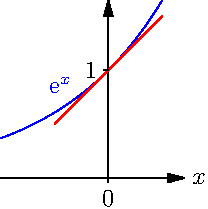
\includegraphics[height=4cm]{expeps}}\pauseb
  \item But $\e{x+\epsilon} = \e{x}\,\e{\epsilon} = \e{x}(1+\epsilon +
    O(\epsilon^2))\pauseb = \e{x} + \epsilon\,\e{x}+ O(\epsilon^2)$\pauseb
    \begin{align*}
      \frac{\dd \e{x}}{\dd x} = \lim_{\epsilon\rightarrow 0}
      \frac{\e{x+\epsilon}-\e{x}}{\epsilon}\pauseb
      =  \lim_{\epsilon\rightarrow 0} \frac{\epsilon\,\e{x} +
      O(\epsilon^2)}{\epsilon} = \e{x}\pauseb
    \end{align*}
  \end{itemize}
\end{PauseHighLight}

\end{slide}

%%%%%%%%%%%%%%%%%%%%%%% Next Slide %%%%%%%%%%%%%%%%%%%%%%%

\begin{slide}
\section[-1]{Functions of Exponentials}

\begin{PauseHighLight}
  \begin{itemize}
  \item What about $f(x)= \e{c\,x}$
    \begin{align*}
      \frac{\dd \e{c\,x}}{\dd x} = c\, \frac{\dd \e{c\,x}}{\dd c\,x} \pause=
      c\, \lim_{c\,\delta x\rightarrow} \frac{\e{c\,x + c\,\delta x} -
      \e{c\,x}}{c\,\delta x} \pauseb =  c \, \e{c\,x}\pauseb
    \end{align*}
  \item This also follows from the chain rule
    \begin{align*}
       \frac{\dd \e{g(x)}}{\dd x} = g'(x)\,\e{g(x)}
    \end{align*}
    if $g(x)= c\,x$ then $g'(x)=c$\pauseb
  \item Also $a^{b\,c} = (a^b)^c$ (that is we multiply $a$
    together $b\times c$ times)\pauseb
    \begin{align*}
      \frac{\dd a^x}{\dd x} = \frac{\dd (\e{\ln(a)})^x }{\dd x}\pauseb =
      \frac{\dd \e{\ln(a)\, x}}{\dd x}\pauseb = \ln(a)\,  \e{\ln(a)\, x}\pauseb =
      \log(a)\, a^x\pauseb
    \end{align*}
  \end{itemize}
\end{PauseHighLight}

\end{slide}

%%%%%%%%%%%%%%%%%%%%%%% Next Slide %%%%%%%%%%%%%%%%%%%%%%%

\begin{slide}
\section{Natural Logarithms}

\begin{PauseHighLight}
  \begin{itemize}
  \item The natural logarithm is defined as the inverse of $\e{x}$
    \begin{align*}
      \ln(\e{x}) &= x  & \e{\ln(y)} =y\pause
    \end{align*}
  \item Recall that if $g(y)= f^{-1}(y)$ then $g'(y) =
    1/f'(g(y))$\pause
  \item Consider $g(y)=\ln(y)$ and $f(x)= \e{x}$ (with $f'(x)=\e{x}$)
    \begin{align*}
      \frac{\dd \ln(y)}{\dd y} = \frac{1}{\e{\ln(y)}}\pause = \frac{1}{y}\pauseb
    \end{align*}
  \item The main feature of any logarithm is that
    \begin{align*}
      \log(0) &= 1 \pause
      &
        \log(a\,b) &= \log(a) + \log(b) \pauseb
      &
        \logg{\frac{a}{b}}&= \log(a) -\log(b) \pauseb
      &
        \logg{a^b} = b\, \log(a)
    \end{align*}
  \item Throughout the lecture course I have used $\log(x)$ to denote
    $\ln(x)$\pause
  \end{itemize}
\end{PauseHighLight}

\end{slide}

%%%%%%%%%%%%%%%%%%%%%%% Next Slide %%%%%%%%%%%%%%%%%%%%%%%

\begin{slide}
\section{Properties of Logarithms}

\begin{PauseHighLight}
  \begin{itemize}
  \item There are many logarithms defined as the inverse of an exponent
    \begin{align*}
      \log_a(a^x) &=x & a^{\log_a(x)}= x \pause
    \end{align*}
  \item Because $a^0 =1$ then $\log_a(1)= \log_a(a^0) = 0\,\log(a)=
    0$\pause
  \item We can write $b = a^{\log_a(b)}$ so
    \begin{align*}
      \log_a\bra{b^c} = \log_a\bra{(a^{\log_a(b)})^c}\pause =
      \log_a\bra{a^{c\,\log_a(b)}}\pauseb = c\,\log_a(b)
    \end{align*}
  \item Since $a^b \, a^c= \logg{a^{b+c}}$
    \begin{align*}
      \logg{a^b \, a^c} = (b+c)\,\log(a)
    \end{align*}
  \end{itemize}
\end{PauseHighLight}


\end{slide}



\message{ !name(calculus.tex) !offset(-359) }
